\chapter{Results} \label{cpt:Results}

This Chapter will discuss the outcome of the programming implementation discussed in previous chapters. The ``outcome'' will be presented using numerous option pricing examples based on our package, as well as some comments on the effectiveness of the result.

The second part of the chapter will discuss the limitations of the package and potential directions of furture development.

\section{Examples} \label{sec:examples}

This section gives demonstration of options pricing via \mintinline{R}|rmcop| package. The installation of the package can be found in the README.md file in Appendix \ref{apd:source_code}. An alternative source would be the GitHub repository page which can be found \hyperref{https://github.com/ZhaiJason/rmcop}{site}{rmcop GitHub repository}{here}.

The following examples assumed users have \mintinline{R}|rmcop| installed and attached. Their device and software configuration should also be suitable (see Section \ref{sec:machine_env} for reference) to running the package.

Prior to running any of the following programmes, users shall ensure that they have attached \mintinline{R}|rmcop| to their current environment, such as using the command:

\begin{Rminted}
library(rmcop)
\end{Rminted}

\subsection{Defining Option and Environment Objects}

As mentioned in Section \ref{sec:Pkg Structure}, \mintinline{R}|"option"| and \mintinline{R}|"env"| class objects are defined using functions \mintinline{R}|option| and \mintinline{R}|option.env|, respectively.

For example, if we want to define an \textit{knock-out Barrier European call option} with strike price 20, maturity of 1 year, barrier of 10, we can use the following command:

\begin{Rminted}
option(
    # Common arguments for the father class "option"
    style = "european", type = "call", option = "barrier", K = 20, t = 1,
    # Arguments for the subclass "barrier option"
    barrier = 10, is.knockout = TRUE
)
\end{Rminted}

And the result S3 list would be:

\begin{Rminted}
> $style
> [1] "european"
> 
> $type
> [1] "call"
> 
> $K
> [1] 20
> 
> $t
> [1] 1
> 
> $barrier
> [1] 10
> 
> $is.knockout
> [1] TRUE
> 
> attr(,"class")
> [1] "barrier" "option" 
\end{Rminted}

If we wish to define an option of other type, style, or family, simply adjusted the ``common'' arguments and specify additional subclass-specific arguments for exotic options.

To define an \mintinline{R}|env| class object, for example, a market environment where the current price is 30, interest rate 0.03, dividend yield rate of 0.02, and volatility rate of 0.01 can be defined using the code below:

\begin{Rminted}
option.env(S = 30, r = 0.03, q = 0.02, sigma = 0.01)
\end{Rminted}

\subsection{Black-Scholes}

\mintinline{R}|rmcop| only supports Black-Scholes formula pricing for vanilla options\footnote{This includes vanilla European options and American non-dividend bearing call option, as other American options cannot be solved using explicit form}.

Suppose we want to know the price of an vanilla option which is specified as:

\begin{Rminted}
option.vanilla <- option("european", "vanilla", "call", K = 20, t = 1)
\end{Rminted}

To use Black-Scholes method, we can specify the argument \mintinline{R}|method = "bs"| when defining the environment object or when triggering the pricing function.

\begin{Rminted}
# Specified when defining environment
env <- option.env(method = "bs", S = 15, r = 0.5, sigma = 0.1)

# Specified when calling pricing function
price.option(obj = option.vanilla, env = env, method = "bs")
> [1] 2.877561
\end{Rminted}

The result price will then be returned after calling the pricing funtion.

\subsection{Binomial Tree} \label{ex:binomial_tree}

The package supports pricing both European and American vanilla options. Similar to the Black-Scholes case, to change the method to using binomial lattice tree pricing, simply specify the argument \mintinline{R}|method = "binomial"| when defining the environment object or calling the pricing function. We will use the exact same option-environment setup as in the prvious section.

Because the binomial tree method used different arguments that the Black-Scholes setup used for Black-Scholes method and Monte Carlo method, when calling the pricing function, users need to specify a few more arguments, including ratios of upward and downward jumps.

\begin{Rminted}
price.option(obj = option.vanilla, env = env, method = "bs")
\end{Rminted}

The below example uses the binomial tree method to price an option under the same steup.

\begin{Rminted}
price.option(
    obj = option.vanilla, env = env, method = "binomial",
    u = 1.2, # Ratio of upward jump
    d = 0.9, # Ratio of downward jump
    n = 10 # Number of steps
)
> [1] 4.166904
\end{Rminted}

The Binomial tree method also allows users to extract more information during the calculation. This can be achieved by specify the argument \mintinline{R}|all = TRUE| in the pricing function.

\begin{Rminted}
# Changed n = 4 for better demonstration
res <- price.option(obj = option.vanilla, env = env, method = "binomial", u = 1.2, d = 0.9, n = 4, all = TRUE)

res$p # Extract the risk-neutral probability
> [1] 0.7771615
res$price_tree # Extract the binomial price tree matrix
>         [,1]   [,2]   [,3]   [,4]   [,5]
> [1,] 15.0000     NA     NA     NA     NA
> [2,] 13.5000 18.000     NA     NA     NA
> [3,] 12.1500 16.200 21.600     NA     NA
> [4,] 10.9350 14.580 19.440 25.920     NA
> [5,]  9.8415 13.122 17.496 23.328 31.104
\end{Rminted}

\subsection{Monte Carlo}

To demonstrate the pricing funciton under the Monte Carlo setup, suppose we are interested in a \textit{binary put option} with strike price 50, maturity of 2 years and payout 10, under a market environment where the current price is 15, interest rate 0.5, and volatility 0.1. We will encode these information using the code below:

\begin{Rminted}
op.binary <- option("european", "binary", "put", K = 50, t = 2, payout = 10)
env <- option.env(method = "mc", S = 15, r = 0.5, sigma = 0.1)
\end{Rminted}

We will price this option-environment combination using Monte Carlo method under the setup of 10000 trajectories simulations, and 1 step only for each trajectory, since a binary option is path-independent.

\begin{Rminted}
set.seed(10)
price.option(op.binary, env, n = 1000, steps = 1)
> [1] 3.487497
\end{Rminted}

Where we will obtain the estimated price.

We can also request for returning more informaiton about the result. For example, we may wish to plot the price trajectories. We can achieve this my simply adding the argument \mintinline{R}|plot = TRUE|.

\begin{Rminted}
# For better demonstration, we set steps = 50
price.option(op.binary, env, n = 1000, steps = 50, plot = TRUE)
\end{Rminted}

This will return us an estimate of the price as well as a result plot of the price trajectory, as shown by Figure \ref{img:example_mc}.

\begin{figure}[H]
    \centering
    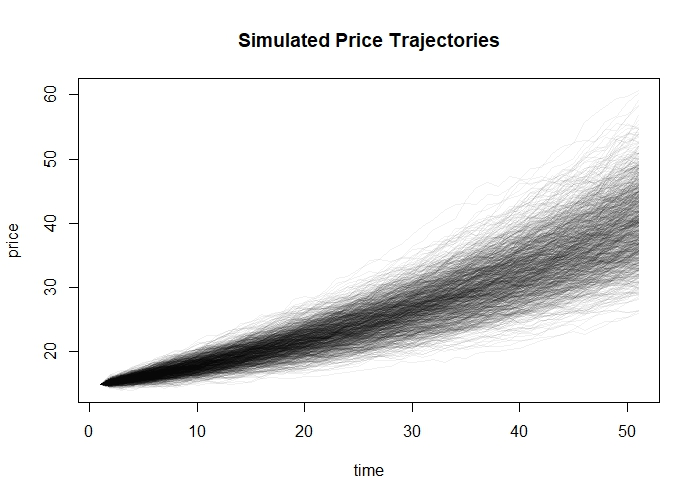
\includegraphics[scale = 0.5]{example_mc.jpeg}
    \caption{Plot of Trajectories} \label{img:example_mc}
\end{figure}

We can also use argument \mintinline{R}|all = TRUE| to store some other useful information (such as option's discounted payoffs) for each simulation\footnote{We see from the first few items of the list that the discounted payoff is either identical or zero (zero cases happens to not be in the head of the vector), which is what we would expect to see from a binary option}.

\begin{Rminted}
res <- price.option(op.binary, env, n = 1000, steps = 1, all = TRUE)
head(res$C) # C is the keyword for extracting option payoffs
> [1] 3.678794 3.678794 3.678794 3.678794 3.678794 3.678794
summary(res$C)
>  Min. 1st Qu.  Median    Mean 3rd Qu.    Max. 
> 0.000   3.679   3.679   3.447   3.679   3.679 
\end{Rminted}

\subsection{Comparing Multiple Option-Environment Setups}

The greatest benefit of encapsulating option and environment characteristics using OOP is that we can compare different setups without adjusting too many arguments.

For example, if we are to compare three different options' prices given the same market condition, shown by the codes below:

\begin{Rminted}
# Defining options of interest
op1 <- option("european", "vanilla", "call", 10, 2)
op2 <- option("european", "vanilla", "put", 12, 2)
op3 <- option("european", "binary", "call", 10, 2, payout = 5)
op.list <- list(op1, op2, op3) # Create a list contining the three options of interest

# Defining the fixed environment
env <- option.env(method = "mc", S = 10, r = 0.05, sigma = 0.01, n = 100000, steps = 1)
\end{Rminted}

We can obtain the result of the three options' corresponding prices by using the \mintinline{R}|lapply| method with just one line of code:

\begin{Rminted}
set.seed(10) # Set seed for random number generator
unlist(lapply(op.list, price.option, env = env))
> [1] 0.9518262 0.8611994 4.5241871

# Equivalently, we can write the pricing function separatedly for each option
price.option(op1, env)
price.option(op2, env)
price.option(op3, env)
\end{Rminted}

We can apply similar methods for cases when comparing different market environment setups. As long as the objects are well defined, one can price any option-environment combinations by simply passing in just two arguments for the \mintinline{R}|price.option| funcitons.

\section{Limitations and Future Development}

Currently, \mintinline{R}|rmcop| only supports a few types of options. The derivative market is varying, and it is infesible for a single package to contain tools that can address all possible scenarios. One of the necessary future development of \mintinline{R}|rmcop| will be extending its support to more cases. This includes the support of pricing American and Bermudian styles options via Monte Carlo method, and the support of more types of exotic options pricing.

There are many additional ways enhancing the accuracy and efficiency of Monte Carlo option pricing that haven't been implemented by this package. For instance, applying variance reduction techniques or quasi-Monte Carlo methods as introduced by Glasserman \cite{Glasserman2003}. Monte Carlo option pricing is a vast topic that is still expanding. The package may consider adding some of these features in later versions.

Though the development of the package includes several R-programming tricks to speed up the computation, one cannot guarantee the implementation here is the most efficient way of encoding the pricing methods. Also, as we discussed in Section \ref{cpt:Existing Packages}, \mintinline{R}|rmcop| being an R-based package has fundamentally no computational advantage comparing to algorithms developed via lower level programming languages. The main focus of this pacakge is for demonstration of model implementations, and the C++ based programmes should be more desirable when conducting more practical and computationally-intensive option pricing projects.

Until the time when this report is completed, the development of \mintinline{R}|rmcop| is still active. One may found resources in Appendix A useful in terms of tracking future updates of the package.

\newpage